\documentclass[tikz,border=2pt]{standalone}
\usepackage{amsmath,amssymb}
\usepackage{pgfplots}
\pgfplotsset{compat=1.18}

\begin{document}
% The Bin(10, 0.3) pmf: the number of successes in 10 independent trials with success
% probability 0.3; the mass peaks around the mean np = 3.
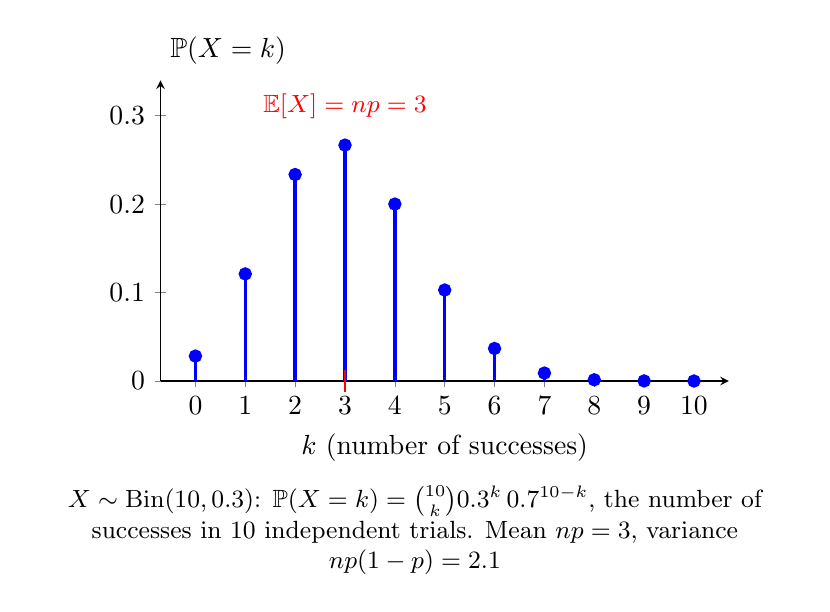
\begin{tikzpicture}
	\begin{axis}[
		axis lines=left, xmin=-0.7, xmax=10.7, ymin=0, ymax=0.34,
		xtick={0,...,10}, ytick={0,0.1,0.2,0.3},
		xlabel={$k$ (number of successes)}, ylabel={$\mathbb{P}(X=k)$}, ylabel style={rotate=-90, anchor=south west, at={(axis description cs:0,1.02)}},
		width=8.8cm, height=5.4cm, clip=false
		]
		\addplot[ycomb, blue, very thick, mark=*, mark size=1.8pt] coordinates {(0,0.0282) (1,0.1211) (2,0.2335) (3,0.2668) (4,0.2001) (5,0.1029) (6,0.0368) (7,0.0090) (8,0.0014) (9,0.0001) (10,0.0000)};
		\node[red, anchor=south, font=\small] at (axis cs:3,0.285) {$\mathbb{E}[X]=np=3$};
		\draw[red, thick] (axis cs:3,-0.012) -- (axis cs:3,0.012);
	\end{axis}
	\node[anchor=north, font=\small, align=flush center, text width=9.6cm] at ([yshift=-2pt]current axis.outer south) {$X\sim\operatorname{Bin}(10,0.3)$: $\mathbb{P}(X=k)=\binom{10}{k}0.3^k\,0.7^{10-k}$, the number of successes in $10$ independent trials. Mean $np=3$, variance $np(1-p)=2.1$};
\end{tikzpicture}
\end{document}
